\documentclass[10pt]{article}
\usepackage[usenames]{color} %used for font color
\usepackage{amssymb} %maths
\usepackage{amsmath} %maths
\usepackage[utf8]{inputenc} %useful to type directly diacritic characters
\usepackage[letterpaper, portrait, margin=1in]{geometry}
\usepackage{graphicx,wrapfig}
\begin{document}
\subsection*{MSDS610 Week 3 HBase Assignment - Nathan Worsham}
\subsection*{Section 2.2}
I started this assignment by powering up my VM from week 1. I decided that I would install the program into the /opt location so I changed to that directory and used wget to gain the install. Finally I extracted the files. 
\begin{figure}[!h]
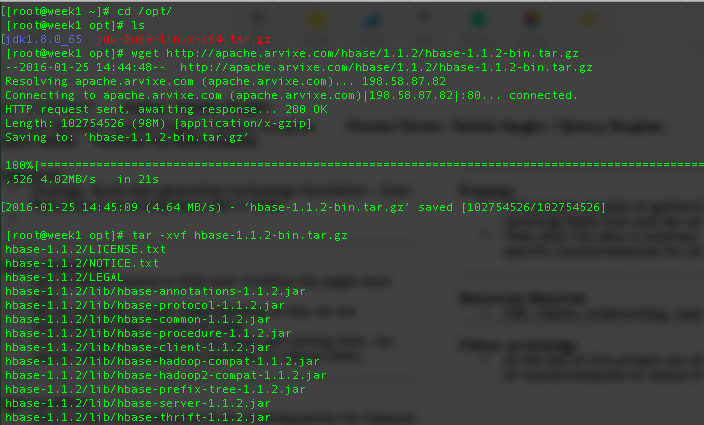
\includegraphics[scale=0.37]{hbase_download.png}
\centering
\end{figure}\\
I set the \verb|JAVA_HOME| in the \verb|/opt/hbase-1.1.2/conf/hbase-env.sh| to what the alternatives command had created a link to: \verb|/usr/bin/java|. I then edited the \verb|conf/hbase-site.xml| file to place the temp data into a directory I can control. Originally I created the directory but then I read that the software would create it so I removed the directory. The instructions where not clear whether or not to provide the "zookeeper" config, but the example had such, so I went ahead and placed that in as well. 
\begin{figure}[!h]
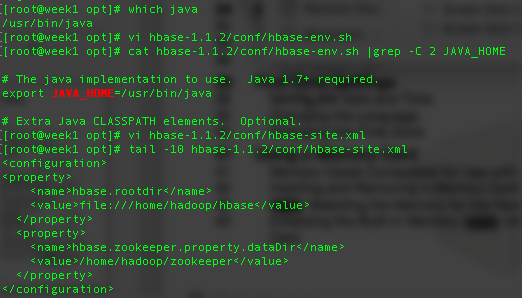
\includegraphics[scale=0.37]{java_env.png}
\centering
\end{figure}\\
Next I tried starting it using the \verb|bin/start-hbase.sh| script but I received several errors. The error that caught my attention the most was that it could not create a log directory. Decidedly my problem here was permissions, as /opt is not generally a directory expected to get written to--usually reserved for /var or /usr (probably where I should have put it in the first place) or /home. I went ahead and elected to move it to the hadoop user's home directory since that was where hadoop was installed on the week 1 assignment and changed the ownership of the folder and it's contents.
\par
\raisebox{-.6\height}{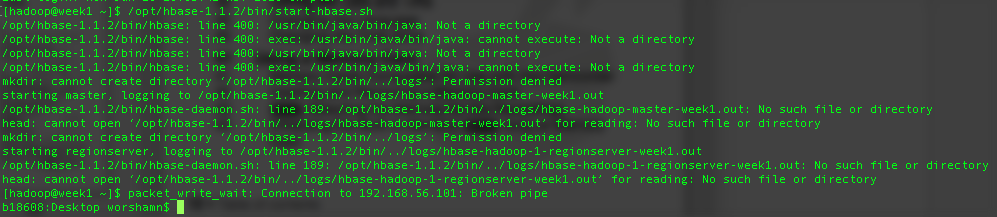
\includegraphics[width=10cm]{start_errors.png}}%
\hfill
\raisebox{-.6\height}{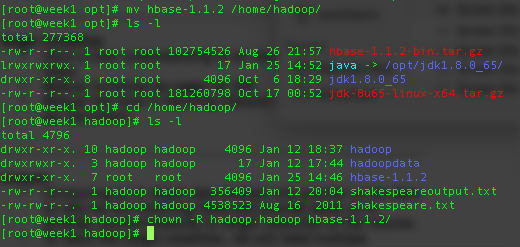
\includegraphics[width=7cm]{move_hbase.png}}%
\par
Now trying to start it again, I received errors about java. Looks like I chose the wrong path for \verb|JAVA_HOME|, so I went ahead and switched it the symbolic link I created for \verb|/opt/jdk1.8.0_65/| which was \verb|/opt/java|. Trying again, this time it starts and jps confirms. There are a couple of warnings about some deprecated options that it went ahead and ignored. 
\begin{figure}[!h]
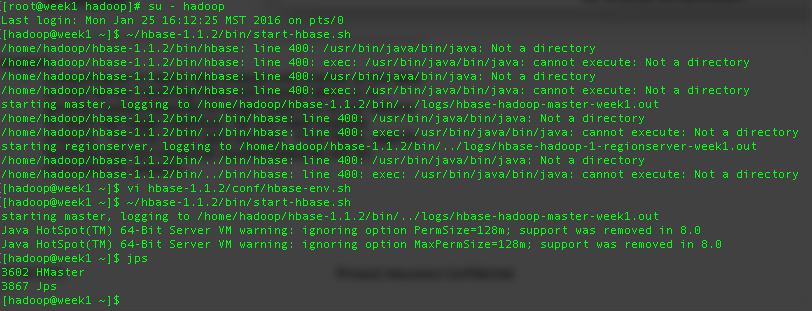
\includegraphics[scale=0.37]{started.png}
\centering
\end{figure}\\
\indent I was successfully able to run the hbase shell and interact with it. I started with creating a table and placing data into it. Then I followed through on their examples of retrieving the data and finally dropping the table.
\par
\raisebox{-.6\height}{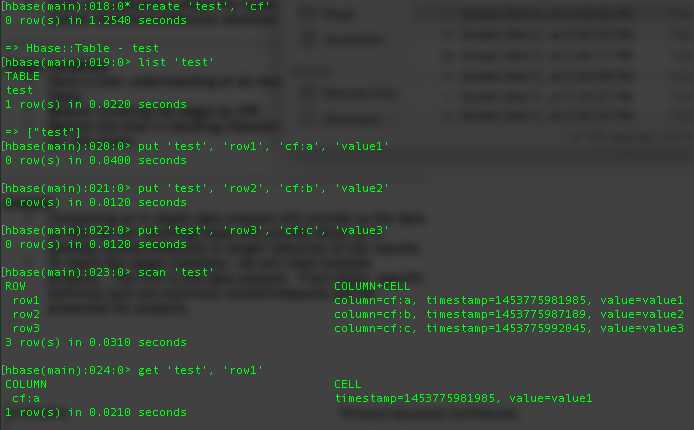
\includegraphics[width=10cm]{create_table.png}}%
\hfill
\raisebox{-.6\height}{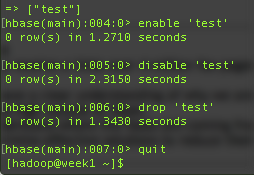
\includegraphics[width=5cm]{drop_table.png}}%
\par
Finally I stopped hbase and confirmed it was no longer running using jps. 
\begin{figure}[!h]
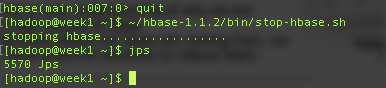
\includegraphics[scale=0.37]{quit_hbase.png}
\centering
\end{figure}\\
\subsection*{Section 2.3}
To start this portion of the assignment I edited the \verb|hbase-site.xml| file to add the clustering option and change the previous root directory for Section 2.2 from local to HDFS. I then started up HDFS.
\par
\raisebox{-.6\height}{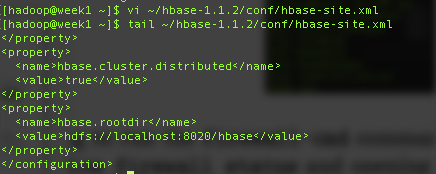
\includegraphics[width=6cm]{hbase_hdfs.png}}%
\hfill
\raisebox{-.6\height}{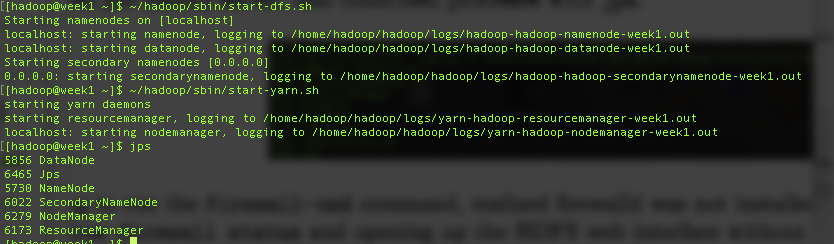
\includegraphics[width=10cm]{start_hdfs.png}}%
\par
I then started hbase and confirmed HRegionServer had started with jps. This looked good but when I did the next check to see if the folder existed in HDFS, I received a "No such file or directory" message. Then looking back on week 1 assignment, it would seem HDFS listens on port 9000 instead of 8020 which is what the documentation asked for. So I made the switch in the conf file and tried starting again, this time I received a message about regionserver already running even though I ran the stop script first. I ran the \verb|ps| command to try to look for it, but the PID number that came up did not match the error message, instead I elected to just reboot the machine and start over.
\begin{figure}[!h]
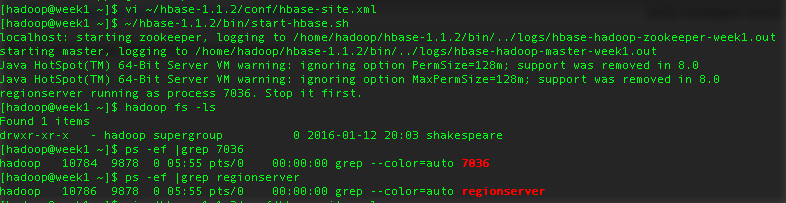
\includegraphics[scale=0.37]{region_running.png}
\centering
\end{figure}\\
\indent After reboot, I again started HDFS and then hbase. This time there was not a complaint about regionserver running and this time running the \verb|hadoop fs -ls /hbase| command actually returned results.
\begin{figure}[!h]
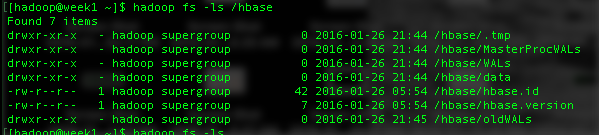
\includegraphics[scale=0.40]{hdfs_working.png}
\centering
\end{figure}\\
I could now enter the hbase shell, albeit took a bit longer to return the shell than it did in the Section 2.2 excercise. I than ran through the same shell exercise as in Section 2.2.
\begin{figure}[!h]
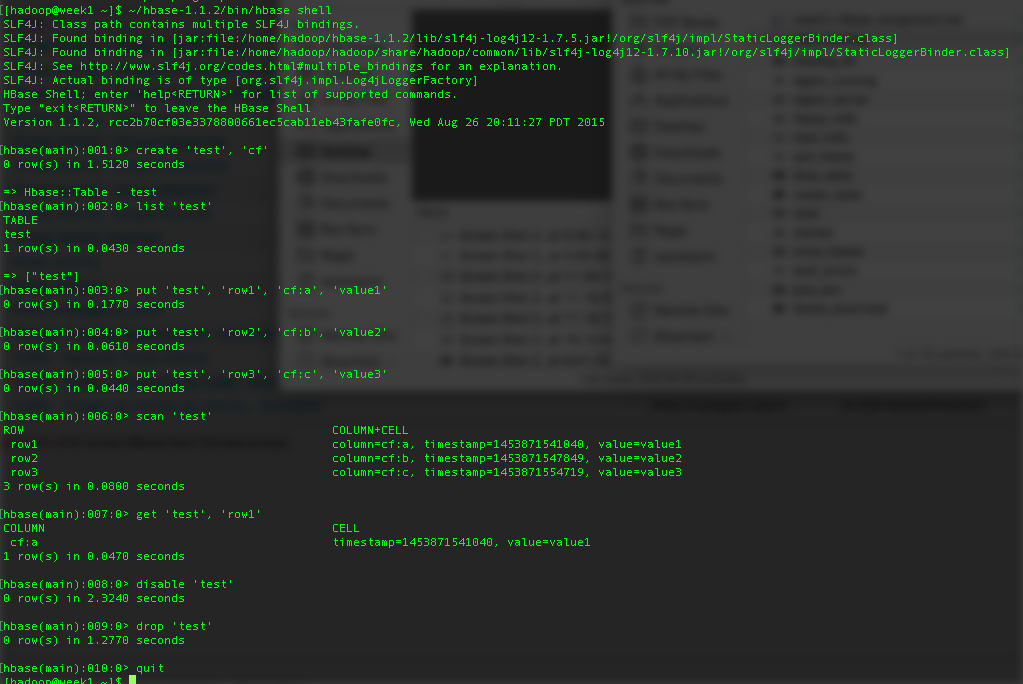
\includegraphics[scale=0.37]{shell_exercise2.png}
\centering
\end{figure}\\
\indent Next the section instructions where to start multiple Hmaster instances. I ran the command it gave \verb|$ ./bin/local-master-backup.sh 2 3 5| but received an error about usage. It would seem that the command wanted start or stop as an argument, so I gave it an argument of "start" before the offset numbers. This time it said it was starting the new Hmasters but when I checked the \verb|/tmp| directory, there where no PID files for the new processes, which could also be seen by trying to stop the processes as it made the same complaint.
\pagebreak
\begin{figure}[!h]
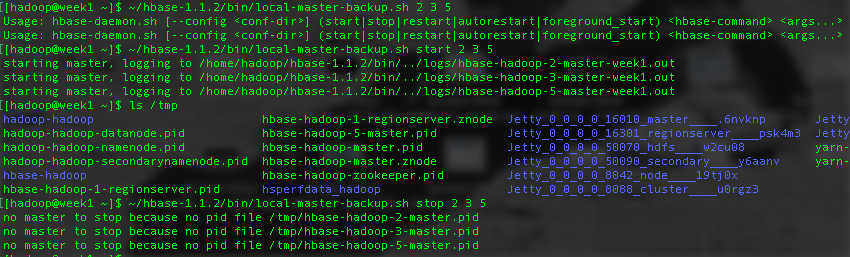
\includegraphics[scale=0.37]{nostart_hmaster.png}
\centering
\end{figure}\\
\indent Looking at the log \verb|/home/hadoop/hbase-1.1.2/logs/hbase-hadoop-2-master-week1.log|, there is an error of "java.net.BindException: Address already in use". But when I use the netstat command (had to install the net-tools package) and grep for 160, I only see the process using 16000 and 16010 and the instructions say that Hmaster would use 16010, 16020, and 16030.
\begin{figure}[!h]
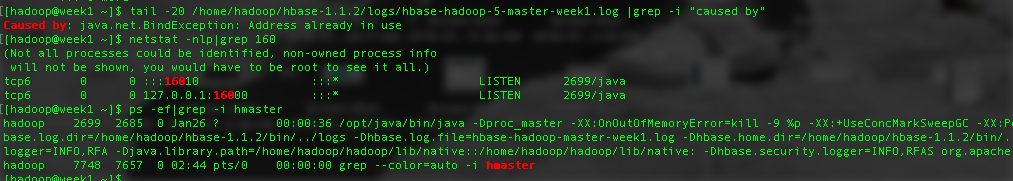
\includegraphics[scale=0.37]{address_inuse.png}
\centering
\end{figure}\\
\indent Running a Google search of "hbase hmaster local-master-backup.sh", surprisingly the very first hit was about not starting Hmaster correctly and an effected version was 1.1.2, whereas version 1.2.0 is fixed. The fix from the JIRA ticket was to add a line to the local-master-backup.sh script: 
\begin{verbatim}
-D hbase.master.port=`expr 16000 + \$DN` \
\end{verbatim}
This makes perfect sense because I found mine running on 16000. I added the line and tried to start it again, this time it did start and then I was able to run the stop command as well.
\begin{figure}[!h]
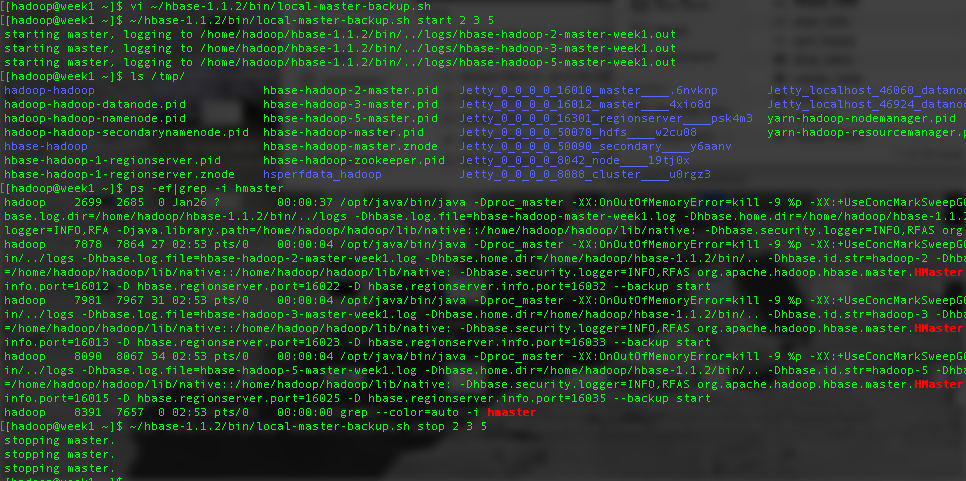
\includegraphics[scale=0.37]{hmasterClust_start.png}
\centering
\end{figure}\\
\indent Finally, I finished out the section running the command to start and then stop additional regionservers and then stopped Hbase.
\pagebreak
\begin{figure}[!h]
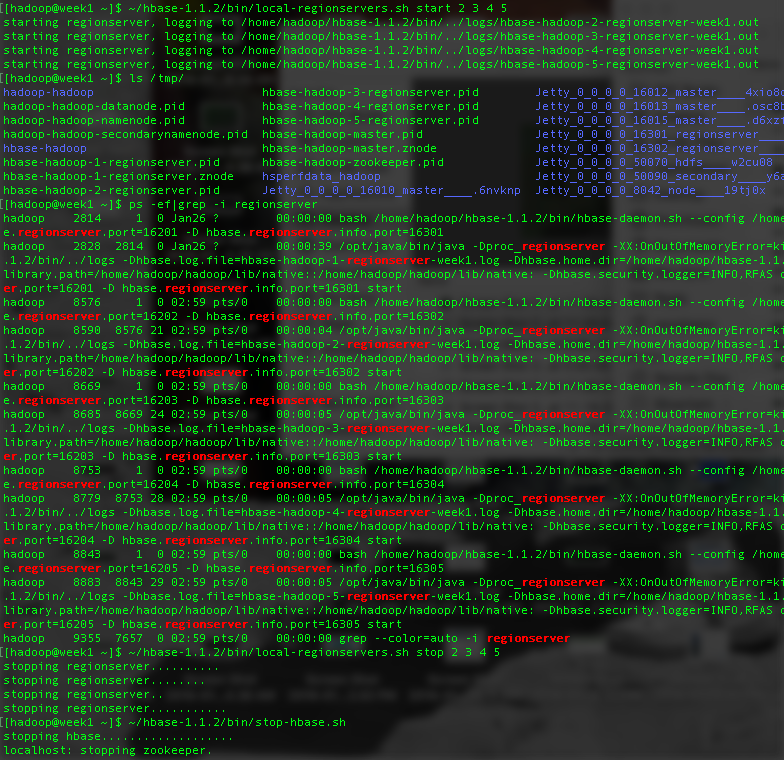
\includegraphics[scale=0.37]{psuedo_end.png}
\centering
\end{figure}\\
\subsection*{Section 2.4}
With this section, I would need to reinstall hbase onto my cluster of VMs created in week 2, but good news is I would be able to skip the steps about ssh key sharing as this was already done last week, though I did still have to copy the keys for node-b (hslave1) to the other nodes since it is the Hmaster backup. In this case I did go ahead and install it into /opt onto 3 of the nodes (I have 4 machines in the cluster but the example was only with three) since that was where hadoop was installed and changed the permissions to the hadoop user. 
\par
\raisebox{-.6\height}{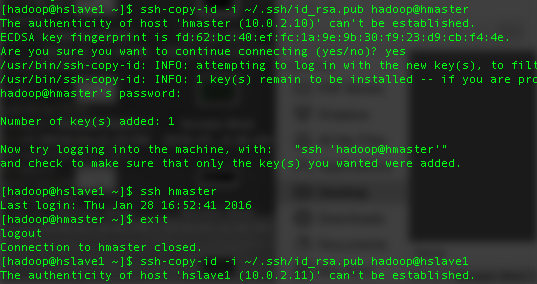
\includegraphics[width=7cm]{copy_keys.png}}%
\hfill
\raisebox{-.6\height}{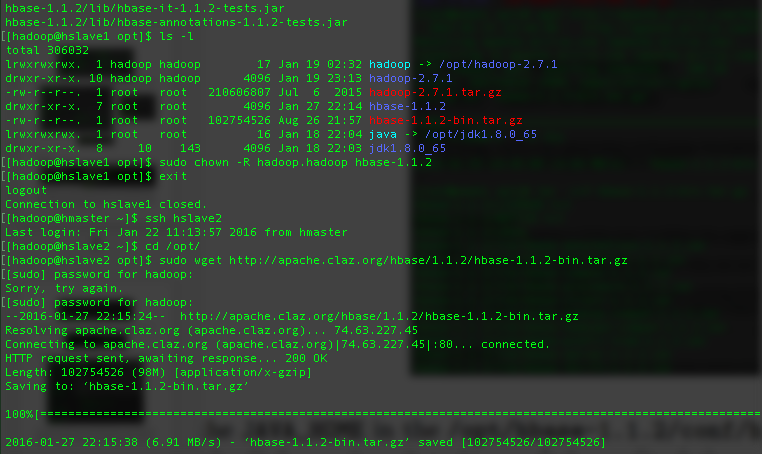
\includegraphics[width=9cm]{cluster_install.png}}%
\par
Since this was not the machine I used for the Section 2.3 exercise I needed to add the HDFS config to the \verb|conf/hbase-site.xml| file. The next step says to change anywhere in the configs "localhost" exists to the name of the node-a but the only place I had it was in the hdfs config pointing to port 9000. It is unclear if in the hadoop cluster if there is only one entry point into the system, but I went ahead and changed it to hmaster and then copied the config to hslave1 and 2. 
\pagebreak
\begin{figure}[!h]
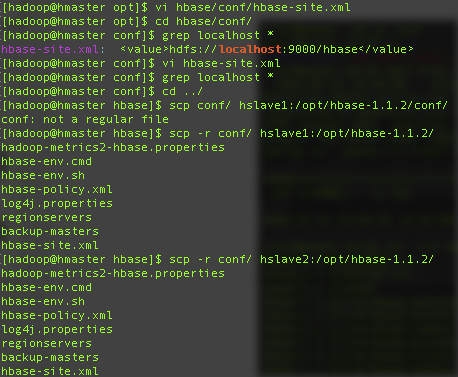
\includegraphics[scale=0.37]{copy_configs.png}
\centering
\end{figure}\\
\indent Before starting Hbase, I first started up HDFS. I then checked that none of the nodes was running any Hbase processes and that HDFS was running with the one-line command:
\begin{verbatim}
for line in $(cat /opt/hadoop/etc/hadoop/slaves);do echo "Host: $line";ssh $line jps;echo " "; done;
\end{verbatim} 
Now I tried starting Hbase with it's start script but received errors about directories not existing on hslave1 or 2:
\begin{verbatim}
hslave1: bash: line 0: cd: /opt/hbase/bin/..: No such file or directory
\end{verbatim}
I realized it was because I had not made a symbolic link on my other 2 nodes. So after correcting the links, I tried starting again this time with success. I now had HMaster running on node-a and node-b, HRegionServer running on node-b and node-c, and HQuorumPeer running on all three. After looking at this, I thought it probably would have made sense to make hslave1 node-a in order to spread out the processes running on the 4 machines. I also made a check to the HDFS to make sure the hbase folder had been created.
\begin{figure}[!h]
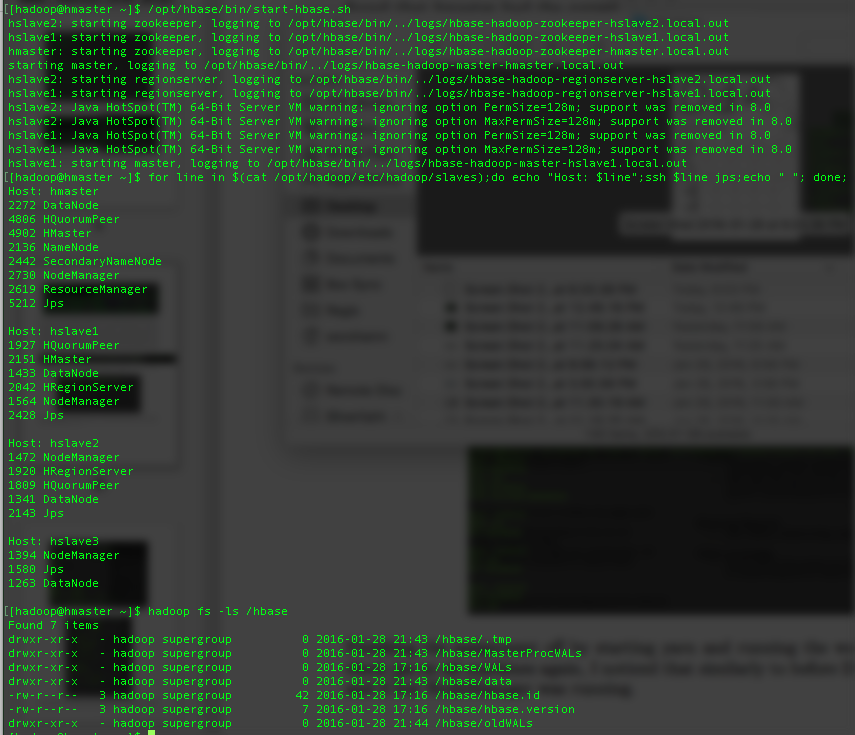
\includegraphics[scale=0.37]{superClust_start.png}
\centering
\end{figure}\\
\indent Unfortunately similarly to my experience last week, though the cluster looked good at startup, it closes down shortly. I found this out when I tried to follow the next step and go to the http page node-a was supposed to have. When I ran \verb|jps| again, the only thing left of hbase I had running was HQuorumPeer. Looking in some of the logs, there were many errors about Zookeeper I just went ahead and elected to stop all services and restart all of the machines and try again. This time I was successful at getting to the website.\\
\begin{figure}[!h]
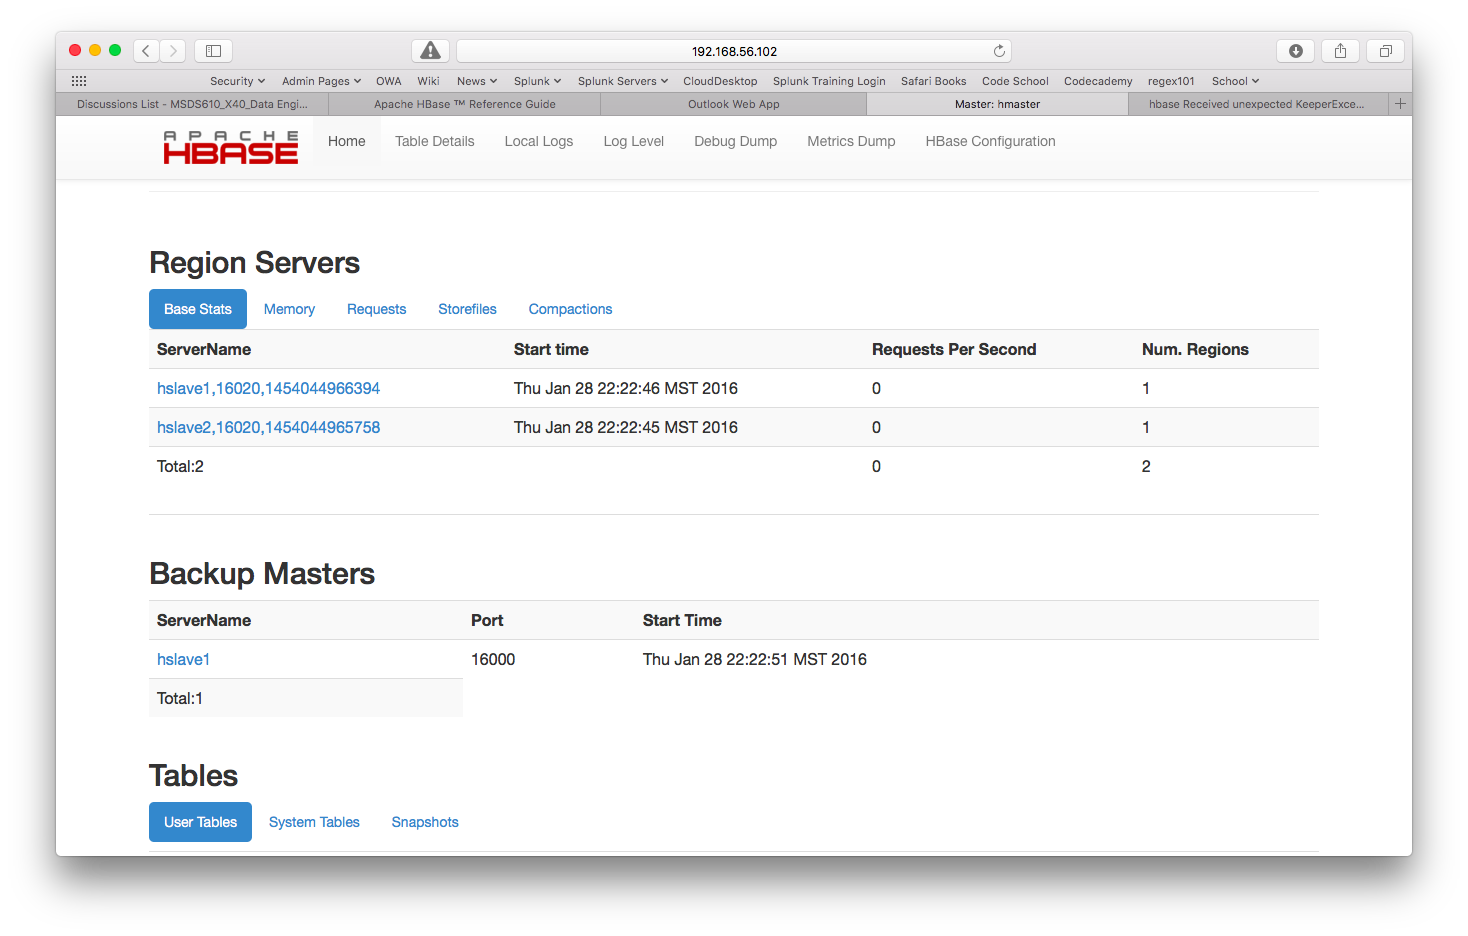
\includegraphics[scale=0.30]{hbase_site.png}
\centering
\end{figure}\\
\subsection*{References}
hbase.apache.org, 2016. Retrieved from http://hbase.apache.org/book.html\#quickstart\\
issues.apache.org, 2016. Retrieved from https://issues.apache.org/jira/browse/HBASE-15057
\end{document}
